\section{Theory}\label{sec:theory_section}
In order to solve the problems introduced in Section~\ref{sec:introduction_section}, effective methods have to be exploited to provide reliable results. Particularly, this paper focused on pursuing the research quest with one specific algorithm, known in the literature as Multidimensional Scaling (MDS) algorithm. \par

The algorithm, as will be later explained, uses the knowledge of relative distances among the set of points, or set of UAVs in this case, to correctly estimate the pose in space and obtain the correspondent Cartesian coordinates. The approach, however, suffers from ambiguity problems that can be solved only if a minimum of $n + 1$ measurements are taken, with $n$ dimension of the search space. Since the same amount of information is needed for computing the classical trilateration algorithm, this will be directly compared to MDS to highlight what might be the benefits or downside for introducing a more complex but robust algorithm.

\subsection{Trilateration algorithm}\label{sec:trilateration}
Trilateration is a geometric methodology that allows to determine the precise spatial coordinates of an unknown point within a given dimensional space, typically 2D or 3D, through the utilization of distance measurements from predetermined reference points. Particularly, the method relies on $n+1$ reference points, known in the literature as anchors, with $n$ dimension of the search space. \par

In details, this algorithm introduces circumferential boundaries, represented as spheres in 3D or circles in 2D, centered at each reference point. The respective radius corresponds to the measured distances. The point of interest is subsequently localized as the intersection juncture of these circumferences or spheres. \par


Given $X_i$ the unknown coordinates of the $i$-th node to be located and, $Q_j$ the coordinates of the $j$-th anchor and $d_{i,\,j}$ the distance between $X_i$ and $Q_j$, the trilateration problem can be solved via LSM by minimizing the loss function reported in Equation~\ref{eq:LSE_equation}.


\begin{equation}
    \label{eq:LSE_equation}
    \hat{X_i} = \min_{X_i} \sum_{j=1}^{n} \left( ||X_i - Q_j|| - d_{i,\,j} \right)^2
\end{equation}

Even though the algorithm is simple, fast and effective, its performances decrease rapidly if incorrect information are introduced, as there is no validation nor correction of noisy measurements. Additionally, if the anchors are absent or the positions of the anchors are not available, the algorithm cannot be applied \cite{Li2021CooperativeNodes}. \par

Figure~\ref{fig:trilateration} provides a visual representation of the just discussed algorithm: it is possible to observe 4 different spheres spotting the unknown point. The respective radii are the measured distances.

\begin{figure}[!ht]
    \centering
    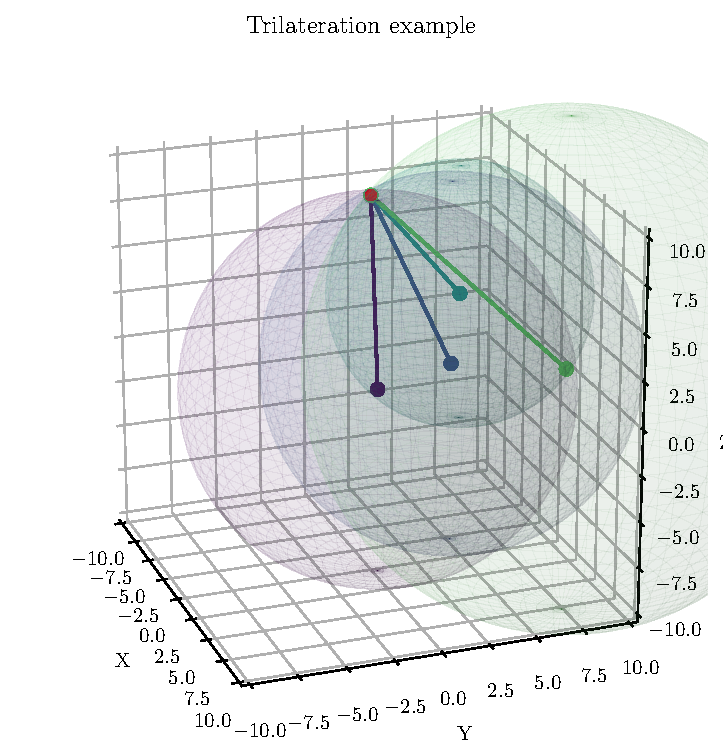
\includegraphics[width=0.4\textwidth]{figures/trilateration.pdf}
    \caption[Trilateration example.]{\textbf{Trilateration example.} 4 spheres detecting an unknown point in space, respecting the $n+1$ rule. The targeted point is found as the intersection of spheres, with no ambiguities.}
    \label{fig:trilateration}
\end{figure}


\subsection{Multidimensional Scaling algorithm}\label{sec:MDS}
MDS is a robust methods that allows to estimate points coordinates given the relative distances among them. Since it relies on fully-connected points, the algorithm results to be robust against noise, as one information, i.e. distance, is validated by another one. Indeed, given two generic points $X_i$ and $X_j$, the distance information $d_{i,\,j}$ obtained from the $i$-th point is supported by the distance $d_{j,\,i}$ read from the $j$-th point. In this way, the method is less dependent on the single piece of information that might be inaccurate, leading to a more balanced solution. Figure~\ref{fig:MDS_visualization} shows an example of fully-connected network of points, in which each node exchanges distance information with the others.\par

\begin{figure}[!ht]
    \centering
    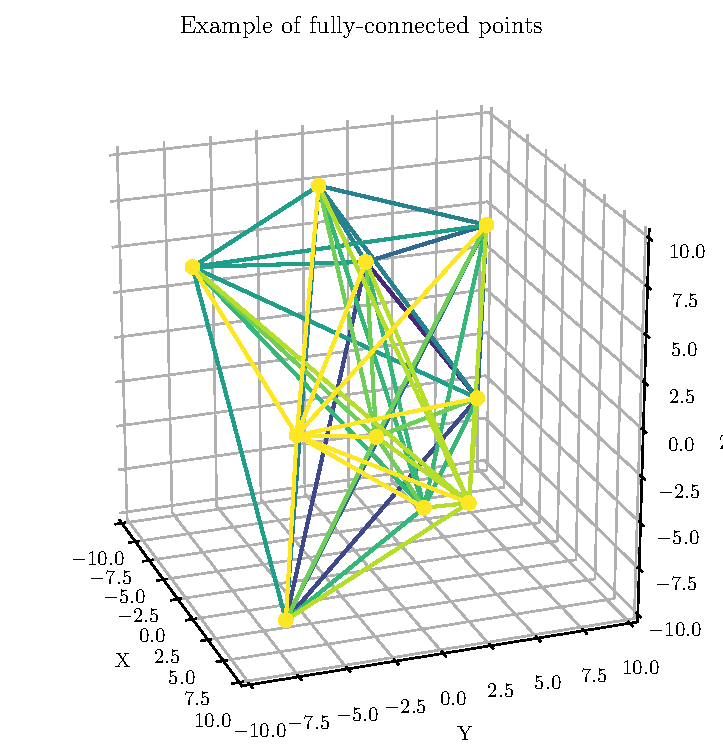
\includegraphics[width=0.4\textwidth]{figures/MDS_visualization.pdf}
    \caption[Example of fully-connected network.]{\textbf{Example of fully-connected network.} Each point communicates with the others, exchanging distance information. The Latin Hypecube Sampling was used for maximizing the distribution of points for this representation. The represented scenario is the input for the MDS algorithm.}
    \label{fig:MDS_visualization}
\end{figure}

The algorithm can be exploited for several applications, but a natural application lies in the estimation of the location of points in space. Specifically, it uses a square matrix of squared distances to build a relative map that describes the distribution of points in space  \cite{Li2021CooperativeNodes}. An example of distance matrix is reported in Equation~\ref{eq:distance_matrix_example}. In details, $d_{i,\,j}$ represents the squared distance between point $i$ and point $j$. Naturally, $d_{j,\,i}$ represents the squared distance between point $j$ and point $i$. In an error- and noise-free scenario, $d_{i,\,j} = d_{j,\,i}$ whilst in a real-case application the two elements might differ due to background noise, latency or interference. \par

\begin{equation}
    \label{eq:distance_matrix_example}
    D = 
    \begin{bmatrix}
    d_{1,1} & d_{1,2} & \dots & d_{1,N} \\
    d_{2,1} & d_{2,2} & \dots & d_{2,N} \\
    \vdots & \vdots & \ddots &  \vdots & \\
    d_{N,1} & d_{N,2} & \dots & d_{N,N} \\
    \end{bmatrix}
\end{equation}

The algorithm results to be easy and flexible and can be summarized in two major steps: \textit{1)} estimation of a relative map from the distance matrix and \textit{2)} transformation of the relative map in the absolute one. The following paragraphs better describe the two steps.\par

\subsubsection{From distance matrix to relative map}\label{sec:from_d_to_rel_map}
The core of MDS relies on the eigendecomposition of a symmetric matrix $D$ of square distances to estimate the relative map of the involved points. \par

Given the $D$ matrix, it is possible to write the associated eigendecomposition by introducing the centering operator $\textbf{H} = \textbf{I} - \textbf{ee}^T/N$, with $N$ dimension of the matrix. The new centered matrix is reported in the left-hand side of Equation~\ref{eq:eigendecomposition}, while the associated decomposition on its right-hand side.

\begin{equation}
    \label{eq:eigendecomposition}
    -\frac{1}{2}\textbf{H}\textbf{D}\textbf{H} = \textbf{U} \boldsymbol{\Lambda}\textbf{U}^T
\end{equation}

Eventually, the relative map $\Tilde{X}$ can be estimated by computing

\begin{equation}
    \Tilde{X} = \boldsymbol{\Lambda}^\frac{1}{2}\textbf{U}^T
\end{equation}

The relative map is a map that describes the location of points in space. It might be affected by unknown Cartesian transformation such as translation, rotation and flip. The fact that a relative configuration can correspond to multiple absolute ones has been called in the literature ambiguity.

\subsubsection{From relative to global map}
In order to turn a relative map to a global map, i.e. the correct estimation of the involved nodes, the ambiguities introduced in Section~\ref{sec:from_d_to_rel_map} must be completely solved. 
In order to achieve that, at least $n+1$ points with known location have to be used. \par

Several methods are known in the literature to solve such problem. Most of them are explained in details in \cite{RisteskaStojkoska2014NodesAlgorithm}. However, thanks to its reliability and accuracy, the Singular Value Decomposition (SVD) method has been chosen for this application, and the following paragraph will explain it in details. \par

Let $p = \left[p_1, p_2, \dots, p_{n+1}\right]$ and $q = \left[q_1, q_2, \dots, q_{n+1}\right]$ two sets of corresponding anchors, where $q$ represents the set of true coordinates and $p$ the estimated one coming out from the eigendecomposition step.

\begin{enumerate}
    \item Compute the weighted centroids of both point sets
    \begin{equation}
        \Bar{p} = \frac{1}{n+1} \sum_{i=1}^{n+1} p_i \text{,}\quad \Bar{q} = \frac{1}{n+1} \sum_{i=1}^{n+1} q_i
    \end{equation}

    \item Compute the centered vectors
    \begin{equation}
        p_i' = p_i - \Bar{p} \text{,}\quad q_i' = q_i - \Bar{q}\text{,}  \quad \forall i \in \left[1, n+1\right]
    \end{equation}

    \item Compute the $n\times n$ covariance matrix
    \begin{equation}
        C =  P' {Q'}^T
    \end{equation}
    where $P'$ and $Q'$ are the $n \times (n+1)$ matrices that have $p_i'$ and $q_i'$ as their columns, respectively.

    \item Compute the singular value decomposition
    \begin{equation}
        C = U\Sigma V^T
    \end{equation}
\end{enumerate}

The unknown rotation can be obtained as
\begin{equation}
    R = V U^T
\end{equation}

while the unknown translation as
\begin{equation}
    t = \Bar{q} - R\Bar{p}
\end{equation}

Therefore, the global map can be written as
\begin{equation}
    \hat{X} = R \Tilde{X} + t
\end{equation}

Please note that with the SVD method, no flip ambiguities must be solved.

% \begin{algorithm}
%     \caption{Multi-Dimensional Scaling algorithm}\label{alg:MDS}
%     \begin{algorithmic}
%     \State{\textbf{Result:} Estimated location of nodes}
%     \State{Initialization}

%     \State Read distances and send information over the network
%     \State Assemble the distance matrix
%     \State Center the matrix
%     \State Compute relative map via Eigendecomposition
%     \end{algorithmic}
% \end{algorithm}

